\documentclass[12pt]{article}
\usepackage[utf8]{inputenc}
\usepackage[finnish]{babel}
\usepackage{graphicx}
\usepackage{float}
\usepackage{hyperref}
\title{Aineopintojen harjoitustyö: Tietokantasovellus\\Dokumentaatio}
\author{Sandra Luhtaniemi}
\begin{document}
\maketitle
\section{Johdanto}
Harjoitustyön aiheena on lankatietokanta. Tietokannan tarkoitus on tarjota käyttäjälleen väline, jolla pitää kirjaa omistamistaan eri käsityölangoista, näiden materiaalista, paksuudesta ja määrästä. Käyttäjä voi esimerkiksi kohdatessaan kiinnostavan neuleohjeen, hakea ohjeessa mainitun langan ominaisuuksien perusteella tietokannasta ne langat, joilla työ olisi mahdollista toteuttaa, sekä tarkistaa, onko hänellä sitä riittävä määrä. Käyttäjä voi myös muilla perusteilla etsiä tietokannasta lankoja, esimerkiksi vaikkapa kaikki sukkalangat. Käyttäjä voi lisätä tietokantaan uudet lankahankintansa, poistaa langan, tai päivittää sen määrän käytettyään jotakin lankaa. Järjestelmän tavoitteena on helpottaa käsitöiden suunnittelua ja vähentää turhia lankahankintoja.
\\ \ \\
Järjestelmä käyttää PostgreSQL-tietokantaa, se toteutetaan php-ohjelmointikielellä, ja se pyörii Tietojenkäsittelytieteen laitoksen users-palvelimella Apache-palvelimen alla. 
\\
\ \\
\textbf{Käyttötapaukset}\\ 
Käyttäjäryhmät:\\
Tietokannalla on vain yksi käyttäjäryhmä. Käyttäjän on rekisteröidyttävä päästäkseen käyttämään tietokantaa. Tämän jälkeen hän voi lisätä tietokantaan lankojaan ja tarkastella tai suorittaa hakuja omistamistaan langoista. 
\\ \ \\
Käyttäjän käyttötapaukset\\
Rekisteröityminen: Käyttäjä luo ensimmäisellä käyttökerralla itselleen käyttäjätunnuksen ja salasanan.
\\ \ \\
Langan lisääminen: Käyttäjä lisää tietokantaan uuden langan
\\ \ \\
Langan poistaminen: Käyttäjä poistaa tietokannasta langan, jonka on käyttänyt loppuun.
\\ \ \\
Langan määrän päivittäminen: Käyttäjä päivittää langan määrän käytettyään siitä osan.
\\ \ \\
Lankojen tarkastelu: Käyttäjä tarkastelee listaa omistamistaan langoista.
\\ \ \\
Haku ominaisuuden perusteella: Käyttäjä hakee tietokannasta kaikki jollakin ominaisuudella varustetut langat.
\\ \ \\
Omien tietojen muuttaminen: Käyttäjä muuttaa omia tietojaan, esimerkiksi salasanaansa tai nimeään.
\\ \ \\
\begin{figure}[H]
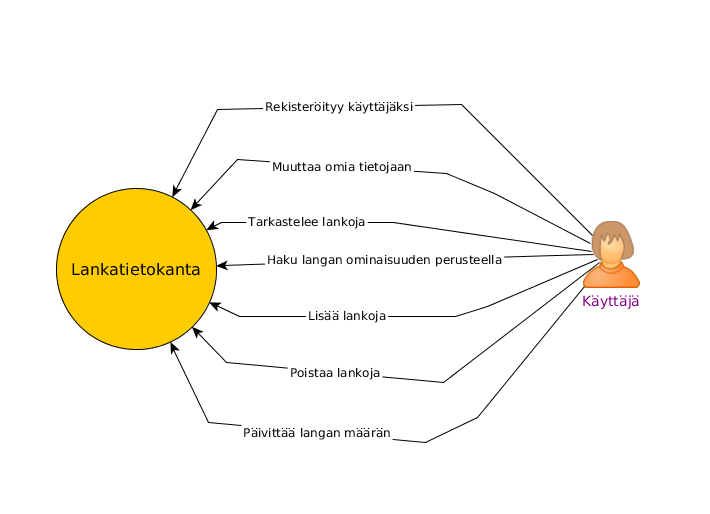
\includegraphics[scale=0.5]{sidosryhmakaavio.png}
\caption{Sidosryhmäkaavio}
\end{figure}
\begin{figure}[H]
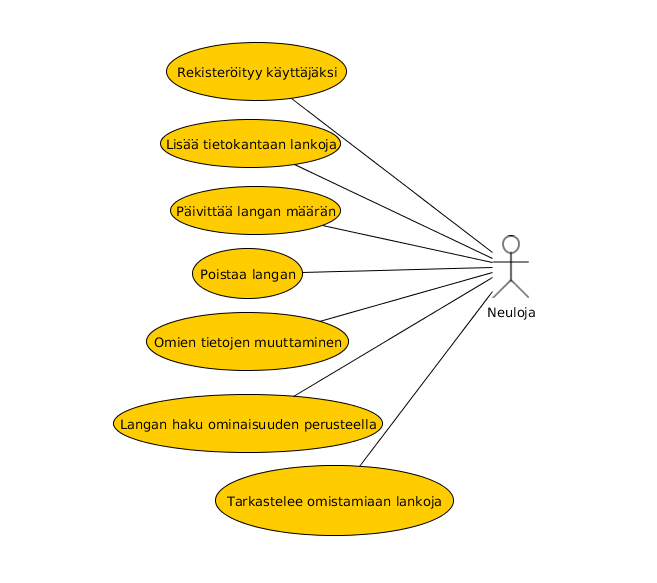
\includegraphics[scale=0.5]{kayttotapaukset.png}
\caption{Käyttötapauskaavio}
\end{figure}

\section{Käyttöliittymän suunnittelu}
Tietokohde: Yarn\\
\begin{tabular}[H]{|c|c|c|}
\hline
Attribuutti & Arvojoukko & Kuvailu \\
\hline
yarnname & Merkkijono & Langan kauppanimi \\
\hline
yarnmanu & Kokonaisluku & Langan valmistajan id-luku\\
\hline
nsrmin & Kokonaisluku & Puikkosuosituksen alaraja kerrottuna 10:llä \\
\hline
nsrmax & Kokonaisluku & puikkosuosituksen yläraja kerrottuna 10:llä \\
\hline
lpg & Kokonaisluku & Sadan gramman sisältämä metrimäärä \\
\hline  
\end{tabular}
\\
Lanka, jolla on jokin puikkosuositus, eli valmistajan antama suositus siitä minkä kokoisilla puikoilla sitä kannattaa neuloa. Puikkosuosituksella on yleensä alaraja ja yläraja, sillä käsiala voi vaihdella neulojasta riippuen. Langalle on ilmoitettu myös metrimäärä, joka sisältyy sataan grammaan, sillä sen avulla voi arvioida langan riittoisuutta.
\ \\ \ \\
Tietokohde: manu\\
\begin{tabular}{|c|c|c|}
\hline
Attribuutti & Arvojoukko & Kuvailu \\
\hline
manuname & Merkkijono & Valmistajan nimi \\
\hline
\end{tabular}
\\
Langan valmistanut yritys.
\ \\ \ \\
Tietokohde:users\\
\begin{tabular}{|c|c|c|}
\hline
Attribuutti & Arvojoukko & Kuvailu \\
\hline
username & Merkkijono & Käyttäjän valitsema käyttäjätunnus\\
\hline
password & Merkkijono & Käyttäjän valitsema salasana\\
\hline   
\end{tabular}
\\
Tietokannan käyttäjä valitsee rekisteröityessään jonkin käyttäjätunnuksen ja salasanan. 
\ \\ \ \\
Tietokohde:attr\\
\begin{tabular}{|c|c|c|}
\hline
Attribuutti & Arvojoukko & Kuvailu \\
\hline
attrname & Merkkijono & langan ominaisuus, esim. väri tai materiaali\\
\hline   
\end{tabular}
\\
Langoilla on erilaisia ominaisuuksia, esimerkiksi väri, materiaali tai vaikkapa huopuvuus tai väriin liityvä erikoisominaisuus, kuten liukuvärjäys. Langalla voi olla useita attribuutteja, ja sama attribuutti voi liittyä useaan eri lankaan. 
\ \\ \ \\
Tietokohde: owns\\
\begin{tabular}{|c|c|c|}
\hline
Attribuutti & Arvojoukko & Kuvailu \\
\hline
amount & kokonaisluku & Kayttajan omistama määrä kyseistä lankaa\\
\hline  
\end{tabular}
\\
Tietokanta voi sisältää monia eri lankoja, mutta käyttäjällä ei välttämättä ole näitä kaikkia tai eri käyttäjillä on lankoja eri määrä. 
\section{Asennusohje}
Tiedostot kopioidaan paikkaan, missä niitä halutaan säilyttää. Tiedostoon lib/settings.php laitetaan asetukset, jolla voidaan muodostaa yhteys tietokantaan. Tietokantaan luodaan taulut ajamalla tiedosto sql/create_tables.sql ja käyttäjä ajamalla tiedosto sql/init_admin.sql. 
\section{Käynnistys- ja käyttöohje}
Tietokanta löytyy osoitteesta \href{http://aluhtani.users.cs.helsinki.fi/tsoha/login.php}{http://aluhtani.users.cs.helsinki.fi/tsoha/login.php}
\\
Kirjautumista ja toimintoja voi kokeilla käyttäjätunnuksella ja salasanalla: ``Anneli'' ja "asdf''.
\section{Järjestelmän yleisrakenne}
Tietokantasovellusta tehdessä on noudatettu MVC-mallia. Kontrollerit ovat juurikansiossa. Näkymät ja malliluokat ovat kansioissa views ja lib. Apukirjastot löytyvät myös kansiosta lib. Asetukset ovat tiedostossa settings.php. Ylläpidon sivuista vastaavissa tiedostoissa on admin-etuliite. Kaikki tiedostonimet on kirjoitettu pienellä. 
\section{Järjestelmän komponentit}
index.php\\
Siirtää käyttäjän sovelluksen sisäänkirjautumissivulle.\\
\ \\
login.php\\
Sisältää kentät sisäänkirjautumista varten. Tänne tulee myös linkki käyttäjäksi rekisteröitymistä varten.\\
\ \\
views/login.php\\
Sisältää Kirjautumissivun näkymän.\\
\ \\
logout.php\\
Kirjaa käyttäjän ulos.\\
\ \\
home.php\\
Sisäänkirjautuneen käyttäjän etusivu. Sisältää linkin omien lankojen tarkasteluun. Admin-käyttäjälle näkyy myös linkki hallinnointisivulle.\\
\ \\
views/home.php\\
Sisältää kirjautuneen käyttäjän etusivun näkymän.\\
\ \\
admin\_home.php\\
Hallinnointisivu, joka sisältää linkit lankojen, valmistajien ja ominaisuuksien lisäämiseen, muokkaamiseen ja poistamiseen.\\
\ \\
views/admin\_home.php\\
Hallintosivun näkymä.\\ 
\ \\
admin\_list\_yarns.php\\
Näyttää listan tietokannassa olevista langoista. Admin-käyttäjä voi lisätä, muokata ja poistaa lankoja.\\
\ \\
views/admin\_list\_yarn.php\\
Näkymä, joka listaa tietokannassa olevat langat ja linkit niiden hallinnointiin.\\
\ \\
admin\_yarn.php\\
Sivu, jolla admin-käyttäjä voi lisätä tietokantaan langan, muokata sen ominaisuuksia tai poistaa sen.\\
\ \\
views/admin\_yarn.php\\
Näkymä, joka näyttää yksittäisen langan ominaisuudet ja muokkaus-, poisto- ja lisäystoiminnot.\\
\ \\
admin\_list\_manus.php\\
Näyttää listan tietokannassa olevista valmistajista. Admin-käyttäjä voi lisätä, muokata ja poistaa valmistajia.\\
\ \\
views/admin\_list\_manus.php\\
Näkymä, joka listaa tietokannassa olevat valmistajat.\\
\ \\
admin\_manu.php\\
Sivu, jolla admin-käyttäjä voi lisätä tietokantaan valmistajan, muokata sitä tai poistaa sen.\\
\ \\
views/admin\_manu.php\\
Näkymä, joka näyttää yksittäisen valmistajan muokkaus- lisäys tai poistotoiminnot.\\
\ \\
admin\_list\_attrs.php\\
Näyttää listan langoilla mahdollisesti olevista eri ominaisuuksista. Sisältää linkit ominaiuuden muokkaamiseen, poistamiseen tai uuden ominaisuuden lisäämiseen.\\
\ \\
views/admin\_list\_attrs.php\\
Näkymä, joka näyttää listan tietokannassa olevista eri lankojen ominaisuuksista.\\
\ \\
admin\_attr.php\\
Sivu, jolla admin-käyttäjä voi muokata ominaisuutta, poistaa sen tai lisätä uusia ominaisuuksia.\\
\ \\
views/admin\_attr.php\\
Näkymä, joka näyttää yksittäisen ominaisuuden muokkaus-, poisto- ja lisäystoiminnot.\\
\ \\
user\_list\_owns.php\\
Näyttää listan käyttäjän omista langoista ja näiden grammamääristä. Käyttäjä voi lisätä kokoelmaansa langan, muokata sen määrää tai poistaa sen kokoelmastaan.\\
\ \\
views/user\_list\_owns.php\\
Näkymä, joka listaa käyttäjän omistamat langat ja näiden määrät.\\
\ \\
user\_yarn.php\\
Sivu, jolla käyttäjä voi muokata kokoelmassaan olevan langan määrää tai lisätä langan kokoelmaansa.\\
\ \\
views/user\_yarn.php\\
Näkymä, joka näyttää yksittäisen langan ominaisuudet, langan poisto- sekä määrän muokkaustoiminnot.\\
\ \\
lib/class\_attr.php\\
Sisältää luokan Attr määrittelyn ja getterit sekä funktiot addAttr, listAttrs, updateAttr, getAttrbyId ja deleAttr.\\
\ \\
lib/class\_manu.php\\
Sisältää luokan Manu määrittelyn, getterit ja funktiot addManu, listManus, updateManu, addManu, deleteManu, getManubyId.\\
\ \\
lib/class\_yarn.php\\
Sisältää luokan Yarn määrittelyn, getterit ja funktiot getYarnByid, setAttributes, listAttributes, listYarns, listYarnsWithManus, addYarn, updateYarn, deleteYarn.\\
\ \\
lib/class\_owns.php\\
Sisältää luokan Owns määrittelyn ja getterit.\\
\ \\
lib/class\_user.php\\
Sisältää luokan User määrittelyn, getterit, ja funktiot isAdmin, owns, insertOwns, updateOwns, deleteOwns, getOwned, amount, getUserByUsername.\\
\ \\
lib/classes.php\\
Lataa kaikki luokat.\\
\ \\
lib/connection.php\\
Ottaa yhteyden tietokantaan.\\
\ \\
lib/lib.php\\
Sisältää erilaisia apufunktioita, joita tarvitaan esimerkiksi eri yhteyksissä, mutta jotka eivät varsinaisesti liity minkään yhden tietyn luokan toimintaan.\\
\ \\
lib/settings.php\\
Sisältää tietokantaan yhdistämiseen tarvittavat asetukset.\\
\ \\
views/template.php\\
Jokaisen sivun näkymän runko.\\
\ \\
views/manufield.php\\
Näkymä joka tulostaa pudotusvalikon eri valmistajista.\\
\ \\
views/nsrfield\\ 
Näkymä, joka tulostaa pudostusvalikot puikkosuosituksista pienimmästä suurimpaan.\\
\ \\
views/yarnfield.php\\
Näkymä, joka tulostaa pudotusvalikon langoista valmistajineen langan lisäämiseksi omaan kokoelmaan.\\
\ \\
views/user\_yarn\_add.php\\
Langan lisäämisessä omaan kokoelmaan käytettävä näkymä.\\
\ \\
views/question.php\\
Näkymä, joka näyttää käyttäjälle kysymyksen ja painikkeita, joilla kysymyksiin voi vastata.\\
\ \\
views/navbar.php\\
Ohjauspalkki, josta käyttäjä pääsee etusivulle, omiin lankoihinsa tai kirjautumaan ulos. Admin-käyttäjä pääsee myös hallintosivulle.\\




\end{document}
